\documentclass[authorversion,nonacm]{acmart}

%\usepackage[hashEnumerators,smartEllipses]{markdown}
\usepackage{pgfplots, pgfplotstable}
\usepackage{url}
\usepackage{tikz}
\usepackage{natbib}
\usepackage{float}
\usepackage{etoolbox}
\usepackage{caption}
\usepackage{subcaption}
\usepackage{listings}
\usepackage{lstautogobble}
\usepackage{xcolor}
\usepackage{balance}
\usepackage{tikz}
\usetikzlibrary{decorations.pathreplacing,calc,shapes,positioning,tikzmark, trees}
\pgfplotsset{compat=1.17}

\renewcommand{\boxed}[1]{\text{\fboxsep=.2em\fbox{#1}}}

\settopmatter{printacmref=false}

\definecolor{darksky}{rgb}{0.4,0.4,1}
\definecolor{skyblue}{rgb}{0.25,0.78,0.96}
\definecolor{lightyellow}{rgb}{1,0.96,0.52}
\definecolor{lightorange}{rgb}{1,0.7,0.4}
\definecolor{lightred}{rgb}{1,0.4,0.4}

\definecolor{codegreen}{rgb}{0,0.6,0}
\definecolor{codegray}{rgb}{0.5,0.5,0.5}
\definecolor{codepurple}{rgb}{0.58,0,0.82}
\definecolor{backcolour}{rgb}{0.95,0.95,0.92}

\lstdefinestyle{python}{
  backgroundcolor=\color{backcolour},   
  commentstyle=\color{codegreen},
  keywordstyle=\color{magenta},
  numberstyle=\tiny\color{codegray},
  stringstyle=\color{codepurple},
  basicstyle=\ttfamily\footnotesize,
  breakatwhitespace=false,         
  belowskip=-0.5em, breaklines=true,                 
  captionpos=b,                    
  keepspaces=true,                 
  numbersep=5pt,                  
  basicstyle=\footnotesize,
  showspaces=false,                
  showstringspaces=false,
  showtabs=false,                  
  tabsize=4
}

\lstset{style=python}

\usetikzlibrary{arrows}

%
%
%


\definecolor{rosso}{RGB}{220,57,18}
\definecolor{giallo}{RGB}{255,153,0}
\definecolor{blu}{RGB}{102,140,217}
\definecolor{verde}{RGB}{16,150,24}
\definecolor{viola}{RGB}{153,0,153}


\tikzset{
  chart/.style={
    legend label/.style={font={\scriptsize},anchor=west,align=left},
    legend box/.style={rectangle, draw, minimum size=15pt},
    axis/.style={black,semithick,->},
    axis label/.style={anchor=east,font={\tiny}},
  },
  pie chart/.style={
    chart,
    slice/.style={line cap=round, line join=round, very thick,draw=white},
    pie title/.style={font={\bfseries}},
    slice type/.style 2 args={
        ##1/.style={fill=##2},
        values of ##1/.style={}
    }
  }
}

\pgfdeclarelayer{background}
\pgfdeclarelayer{foreground}
\pgfsetlayers{background,main,foreground}


\newcommand{\pie}[3][]{
    \begin{scope}[#1]
    \pgfmathsetmacro{\curA}{90}
    \pgfmathsetmacro{\radius}{1}
    \def\Centre{(0,0)}
    \node[pie title] at (90:1.3) {#2};
    \foreach \v/\s in{#3}{
        \pgfmathsetmacro{\deltaA}{\v/100*360}
        \pgfmathsetmacro{\nextA}{\curA + \deltaA}
        \pgfmathsetmacro{\midA}{(\curA+\nextA)/2}

        \path[slice,\s] \Centre
            -- +(\curA:\radius)
            arc (\curA:\nextA:\radius)
            -- cycle;

   % to determine direction of lines (left/right, up/down
   \pgfmathsetmacro{\ysign}{ifthenelse(mod(\midA,360)<=180,1,-1)}
   \pgfmathsetmacro{\xsign}{ifthenelse(mod(\midA-90,360)<=180,-1,1)}

   \begin{pgfonlayer}{foreground}
        \draw[*-,thin] \Centre ++(\midA:\radius/1.1) -- 
                               ++(\xsign*0.1*\radius,\ysign*0.3*\radius) -- 
                               ++(\xsign*\radius,0) 
                      node[above,near end,pie values,values of \s]{$\v\%$};
   \end{pgfonlayer}


        \global\let\curA\nextA
    }
    \end{scope}
}

\newcommand{\legend}[2][]{
    \begin{scope}[#1]
    \path
        \foreach \n/\s in {#2}
            {
                  ++(0, -10pt) node[\s,legend box] {} +(5pt,0) node[legend label] {\n}
            }
    ;
    \end{scope}
}



%
%
%

\AtBeginDocument{%
  \providecommand\BibTeX{{%
\normalfont B\kern-0.5em{\scshape i\kern-0.25em b}\kern-0.8em\TeX}}}

\setcopyright{acmcopyright}
\copyrightyear{2023}
\acmYear{2023}
\acmDOI{10.1145/1122445.1122456}

%% These commands are for a PROCEEDINGS abstract or paper.

\copyrightyear{2023}
\acmYear{2023}
\setcopyright{acmlicensed}\acmConference[SIGCSE 2023]{Proceedings of the 54th ACM Technical Symposium on Computer Science Education V. 1}{March 15--18, 2023}{Toronto, ON, Canada}
\acmBooktitle{Proceedings of the 54th ACM Technical Symposium on Computer Science Education V. 1 (SIGCSE 2023), March 15--18, 2023, Toronto, ON, Canada}
\acmPrice{15.00}
\acmDOI{10.1145/3545945.3569801}
\acmISBN{978-1-4503-9431-4/23/03}

\begin{document}

%\definecolor{rosso}{RGB}{220,57,18}
%\definecolor{giallo}{RGB}{255,153,0}
%\definecolor{blu}{RGB}{102,140,217}
%\definecolor{verde}{RGB}{16,150,24}
%\definecolor{viola}{RGB}{153,0,153}


\title{On the Design and Use of Distractors in Parsons Problems}

\author{David H. Smith IV}

%1-2 page intro  (why should I care?)
%2-3 pages background / related work  (have you done your homework?)
%4-5 pages on previous work  (are you ready to prelim?  will you be successful on future work?)
%4-5 pages on future work  (what are you proposing to do?  why?  how?)
%1 page on schedule  (is your schedule realistic?  will you have done enough to earn a Ph.D.?)

\begin{teaserfigure}
    \centering
    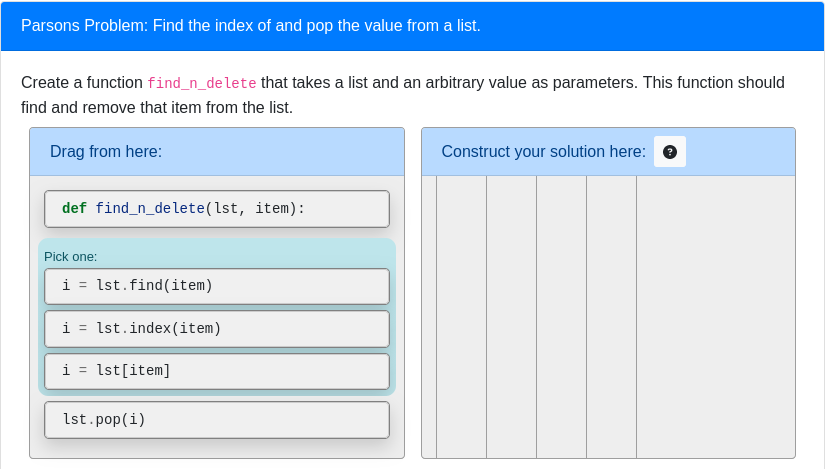
\includegraphics[width=0.70\textwidth]{imgs/parsons.png}
    \caption{Examples of Parsons Problems with Distractors on PrairieLearn}
\end{teaserfigure}

\maketitle

\section{Extended Abstract}

% Very Brief intro to parsons problems.
Since their introduction by \citet{parsons2006parson} distractors have become
common place in studies investigating Parsons problems. However, to date, there
have been a limited number of studies investigating the utility of including
distractors in Parsons problems at all.  In filling this gap, my work thus far
has focused on investigating methods of developing distractors and the impact
of distractors in Parsons problems in a summative context. I first introduce a
method of creating distractor templates from analysis of code writing errors
and using those templates to support the autogeneration of distractors~\cite{}.
I am also currently in the process of integrating this system of distractor
autogeneration into the CodeSpec platform~\cite{}. Since the creation of this
tool, I have conducted a series of studies comparing Parsons problems on exams
that include distractors to those that do not and comparing the use of jumbled
and visually grouped distractors~\cite{}. Furthermore, I have added the ability
to associate feedback with distractors in PrairieLearn. This is done towards
supporting future work in investigating the utility of distractors in formative
activities.

% My proposed future work
My proposed future work can be divide into three main areas of focus: (1)
performing further analysis of common errors made by students in code
writing exercises towards creating a taxonomy of distractors, (2) extending
my prior analysis investigating the impact of using distractors in summative
contexts, and (3) investigating the impacts of distractors in formative contexts.
In doing so, I hope to provide instructors and curriculum designers with a
better understanding of how distractors can be used in designing assessments and
learning activities alike.

\section{Introduction}

% What are parsons' + Distractors
Parsons problems were first proposed by \citet{parsons2006parson} as a method
of facilitating the development of fundamental semantic and syntactic concepts
in introductory programming students. These problems consist of individual
blocks of code that must be arranged in a specific order in order to construct
a valid solution. Code blocks that either contain errors or are not used in the
final solution, commonly referred to as distractors, were introduced in the
original and continue to be included in many studies involving Parsons
problems~\cite{du2020review}.  

% When are distractors used in Parsons and why?
Distractors are often design to reflect common programming errors and
misconceptions~\cite{du2020review, parsons2006parson}.  Much like with
multiple-choice questions, distractor blocks are added to Parsons problems with
the intention of distracting students with plausible, but incorrect
alternatives.  When included on homework assignments the purpose of distractors
is to illustrate and correct common errors and misconceptions students may have
when writing programs without having them deal with the full cognitive load of
writing a program from scratch~\cite{ericson2017solving, haynes2021problem}.
When included on exams, their purpose shifts to providing an additional
dimension by which to discriminate based on student knowledge. As such, the
selection of distractors that accurately reflect common errors is important
when pursuing either of these goals. 

% Where do distractors come from in the context of MC
The design and impact of distractors with respect to multiple-choice questions
has long been a topic of consideration given the widespread usage of this
question format.  As summarized by \citet{gierl2017developing}, designing
distractors is difficult for three main reasons. First, it requires an
experienced individual to write a large number of plausible but incorrect
options.  Next, if distractors are too obviously incorrect it can limit the
amount of thought students must put into answering the question. This, in turn,
limits the learning potential of the question ~\cite{little2015optimizing}.
Finally, the quality of distractors impacts the quality of feedback an
instructor can receive from the question on the misconceptions their class may
hold.

% Where do distractors come from
Though experts may attempt to construct distractors based on their perceptions
of the issues students face when writing a given line of code, expert-blind
spots may make this an unreliable method for generating
distractors~\cite{nathan2001expert}. As such, one of the common methods by
which distractors are created is by collecting common errors or misconceptions
from related short response questions~\cite{briggs2006diagnostic,
halloun1985initial}. Though these are commonly collected from students
responses on test and homework questions, there are other methods by which
these responses can be collected at scale.  For example,
\citet{scheponik2019investigating} found that using open-ended questions posted
on Amazon's Mechanical Turk was a useful method by which to collect distractors
for multiple-choice questions. 

\section{Background}

\subsection{Parsons Problems}

% Origins and types of Parsons problems
The development of ``Parsons Programming Puzzles'' by \citet{parsons2006parson}
was initially aimed at allowing for a more engaging form of the type of
practice drills that are common in other introductory science and engineering
courses. The purpose of those drilling exercises and, by extension the Parsons
problems, is to facilitate the development of fundamental programming concepts
such as being able to correctly identify correct syntax and create logical
constructs.  As such, these programming puzzles were developed with the
following design goals in mind:
\begin{enumerate}
    \item Permitting common syntactic and logical errors.
    \item Addressing misconceptions through immediate feedback.
    \item Modeling good code.
    \item Constraining the logic used to solve a problem.
\end{enumerate}
The combination of permitting common errors through the inclusion of
distractors and providing immediate feedback is used as a method by which
common errors can be addressed in a scaffolded environment.  Parsons problems
have gained traction given their positive reception among students and
instructors alike~\cite{ericson2015analysis, ericson2016identifying}.

% The role of Parsons problems in instruction
In terms of pedagogical utility, the ability of students to solve Parsons
problems has been found to be highly correlated with other skills such as code
writing and tracing suggesting they may employ many of the same
skills~\cite{whalley2007many, lopez2008relationships, venables2009closer,
fowler2022reevaluating}.  \citet{ericson2017solving} compared Parsons problems
that require students to correctly indent blocks, code fixing, and code writing
problems on the basis of efficiency, effectiveness, and cognitive load.
Efficiency was operationalized as the amount of time needed to complete the
problem, effectiveness was the increase in performance between a pre and post
test after completing the set of treatment problems, and cognitive load was
measured using the CS Cognitive Load Component
Survey~\cite{morrison2014measuring}. Their findings indicate that Parsons
problems are both more efficient and require less cognitive load while still
achieving the same learning benefits compared to practicing with code writing
and code fixing exercises.

\subsection{Approaches to Including Distractors}

There are two main ways in which distractors are included in Parsons problems.
The original method simply randomly placed distractors in with correct blocks
and left it to the students to distinguish which they should use, a process 
that would come to be known as \textit{jumbled distractors}.
Prior work has found that including jumbled distractors leads to a decrease in
efficiency and completion while increasing cognitive
load~\cite{garner2007exploration, harms2016distractors} and increasing the
number of distractors made problems more difficult~\cite{ericson2015analysis}.
An alternative involves visually grouping distractors with their correct alternative.
When each group includes a single correct block and a single distractor this is commonly
refered to as ``visually paired distractors''~\cite{} whereas when each correct block
has more than one distractor associated with it this is refered to as
``visually grouped''~\cite{}.  The purpose of visually grouping and visually pairing
is to improve problem efficiency by making the selection between a correct block 
and its distractors more explicit~\cite{denny2008evaluating}.

Beyond the method by which distractors are included 
recent work has investigated the utility of adaptive Parsons, where, 
as students submit incorrect responses, distractors are eliminated and correct
blocks are combined. The purpose of these problems is to progressively morph
the problem to fit the students current ability
level~\cite{ericson2016dynamically, ericson2019investigating}. The purpose of
this is to keep the student in the zone of proximal
development~\cite{vygotsky1978mind}, where students are challenged but still
able to progress rather than stagnating and becoming frustrated. 

\subsection{Role of Distractors in Parsons Problems as Test Items}

% Tee up future work 
Despite the initial purpose of Parsons problems as a type of drilling exercise,
they have also been used as a tool for examination~\cite{ lister2010naturally,
lopez2008relationships}.  \citet{denny2008evaluating} investigated the
correlations between Parsons, code writing, and tracing problems on an
assessment and found a particularly high correlation between students scores on
Parsons and code writing questions, suggesting they measure similar skills.
Additionally, their interviews uncovered several recommendations for designing
Parsons problems as exam questions.  First, each line should have two explicit
options where one is correct and the other is a distractor so as to avoid
extraneous cognitive load. Next, labeling each line with a letter and having
students write the letters in their selected order lead to accidental errors
(e.g., copying the wrong letter) and extraneous cognitive load  when tracking
letter-line mappings. Having students write the lines of code they select is
recommended as an alternative. Finally, cues can be embedded in questions, such
as the placement of brackets or variable names, to help reduce the problem's
difficulty by hinting at the correct solution's structure.  

It is worth noting that all of the previously mentioned studies took place
in the context of paper-based assessments which may alter some of the
considerations presented by previous studies when considering computer-based
exams. For example, the recommendations by \citet{denny2008evaluating} that
students write the responses rather than using letter tags are no longer a
consideration when students can drag and drop blocks on a computer.
Furthermore, the rubrics developed for code writing and Parsons problems might
be altered for automatic grading by using test-cases~\cite{
eddelbuettel2020r} and distance from the correct
solution~\cite{poulsen2022efficient}, respectively. 

% Why good distractors matter
The concept of ``desirable difficulties'' is a major consideration when
constructing test-items and learning activities~\cite{bjork2011making,
bjork2014multiple}.  In the context of multiple-choice questions on exams, the
selection of distractors can impact the retrieval processes necessary to solve
the problem~\cite{little2015optimizing}. The retrieval processes that occur 
during assessments have been associated with increasing retention of the
information on which the student is being tested in what has come to be known
as the ``testing-effect''~\cite{izawa1966reinforcement, rowland2014effect}.  As
such, the selection of effective distractors is not only a concern in
constructing questions that effectively discriminate between high and low
performing students, but they may also play a role in maximizing a given item's
learning potential.

\subsection{Distractors in Multiple-Choice Questions vs Parsons Problems}

Distractors have been most often used and investigated in the context of
multiple-choice and true-false questions where they play a significant role in
determining item quality~\cite{gierl2017developing}. It is often recommended
that instructors include short answer questions on their assessments and use
common incorrect responses to create distractors for future multiple choice
questions~\cite{briggs2006diagnostic}.  Distractors might also come from domain
experts who design distractors to test for specific
misconceptions~\cite{guttman1967systematic}. In general, three distractors and one correct response are
recommended as increasing to three or four has little impact on item difficulty,
discrimination, and validity but a significant impact on the time it takes to
create questions and students' efficiency in answering them~\cite{vyas2008multiple}.

Once distractors are created and administered to students their quality can be
assessed in a variety of ways. First, the item can be taken as a whole and its
discrimination and difficulty can be calculated~\cite{mahjabeen2017difficulty}.
Distractors can then be assessed individually to identify and remove ones that are
selected significantly less than their counterparts or not at all~\cite{tarrant2009assessment}.  Furthermore, a process known as
``Differential Distractor Functioning'' can be used to identify if any
subpopulations are being unfairly disadvantaged by the presence of certain
distractors~\cite{green1989method}.

Despite being included in Parsons problems since their
inception~\cite{parsons2006parson}, similar investigations into how to
effectively create, use, and audit distractors in this context
are limited. \citet{du2020review} suggest in their literature review that, like
multiple choice questions, distractors for Parsons problems should be created to
reflect common misconceptions and errors. Distractors have been investigated in
formative contexts with \citet{harms2016distractors} findings that they decrease
efficiency and success rates while showing no impact on learning compared to
students who practiced problems that did not include distractors. Given these
limited investigations, it remains largely unknown what the impact of distractors
are when used in exam questions and what the best practices are for creating
distractors.


\subsection{Classical Test Theory and IRT}

One of the key methods of evaluating an exam's quality is test reliability,
commonly calculated using Cronbach's Alpha~\cite{cronbach1951coefficient}
(Equation~\ref{fig:cronbach}). 
\begin{equation}
    \alpha =\left({k \over k-1}\right)\left(1-{\sum _{i=1}^{k}\sigma
    _{i}^{2} \over \sigma _{x}^{2}}\right)
\end{equation}\label{fig:cronbach}
At its core, reliability is a measure that identifies the degree to which
items in an exam are interrelated which in turn reflects the degree to which the
assessment measures what it purports to measure~\cite{lord2008statistical,
ebel1967relation, ebel1972essentials}.  
One of the major contributors to the reliability is the number number of items on
the test. As the number of items ($k$) grows so does the reliability, assuming those items can be expected to have
similar properties~\cite{ebel1967relation, allen2001introduction, ebel1972essentials}.
However, as \citet{ebel1967relation} suggests, in practice it is often
unfeasible to increase the size of an assessment to the point of having a
substantial impact on reliability. This leaves 
analysis and improvement of individual items as one of the primary ways in
which instructors can iteratively improve their exam questions with the
intention of reducing the exam score variance ($\sigma^2_x$) an item variance 
($\sigma^2_i$).

Item analysis in Classical Test Theory (CTT) is generally concerned with
assessing items based on two metrics: item difficulty and item discrimination.
Difficulty is operationalized as the proportion of respondents that answer a
given item correctly~\cite{engelhart1965comparison, brennan1972generalized},
often in the context of dichotomously scored items making this functionally
equivalent to average score.  Discrimination, on the other hand, has been
defined in a number of ways.  Traditionally, it is calculated by dividing
students into groups of lower and upper performing groups and finding the difference
between
the proportion of students that responded correctly in the upper group vs the
lower group. In more recent works, a Pearson-product-moment correlation between
item score and test score is more often used for tests that contain questions
with partial credit~\cite{setiawan2014simulation}. A simplification of the
Pearson's correlation known as a point-biserial correlation is often used for
tests that contain only dichotomously scored items~\cite{kornbrot2014point}.
Fundamentally, all measures of item discrimination are attempting to quantify
the relationship between the skills needed to answer the question and the skills
needed to perform well on the assessment as a whole. This makes item discrimination a
metric that identifies which items are most effective at measuring the skill(s)
the test is attempting to measure.  As such, item discrimination is often
referenced as being one of the main indicators of item quality. 
\begin{quote}
    Working to improve the discrimination of the individual items in most
    classroom tests is probably the most effective means of improving score
    reliability and, hence, test quality. - \citet{ebel1972essentials} (pp. 90)
\end{quote}
However, item difficultly and discrimination go hand in hand. If an item is
so hard that everyone gets it incorrect or so easy that everyone gets it correct then that item is unlikely to have high discrimination. For general tests, midrange item difficulties (0.3-0.7)
are often recommended to increase the possible range of scores the item can
produce~\cite{lord1953application, ebel1972essentials, hotiu2006relationship}.
%, though this does vary based on the item type and scoring method TODO: double check this statement with the above citations.

\section{Prior Work}

\subsection{Creation of Distractors and Pilot Study}\label{sec:creation}

\paragraph{Objectives:} In investigating the utility of distractors it became 
apparent that developing a systematic process of creating distractors and 
quickly authoring questions that utilize them would be a required first step.
As an initial step in addressing this gap we make three contributions related to
the selection and use of distractors in Parsons problems. First, we demonstrate
a process by which templates for creating distractors can be selected through
the analysis of student submissions to short answer questions. Second, we
describe the creation of a tool that uses these templates to automatically
generate distractors for novel problems. Third, we perform a preliminary
analysis of how the presence of distractors in Parsons problems being used on
summative assessments impacts: (1) performance, (2) the amount of time students
spend working on the problems, and (3) item quality as measured through
Classical Test Theory's operationalization of item-discrimination.

\paragraph{Methodology:}

\begin{figure}
  \centering
  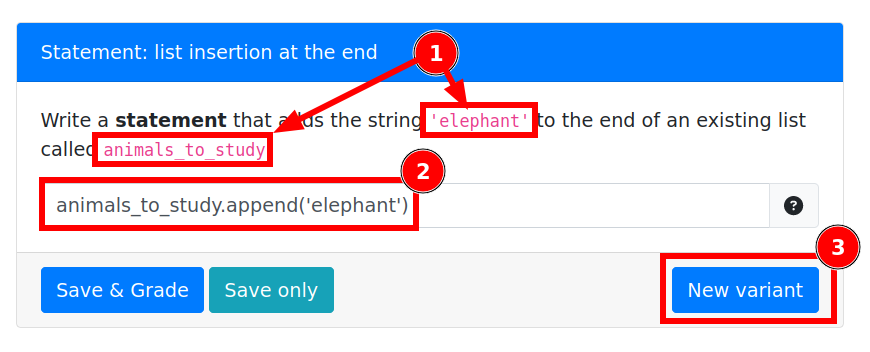
\includegraphics[width=300px]{imgs/pl-question.png}
  \caption{
    An example of a statement question from the course. (1) Elements of these
    questions (e.g., variables, values) are randomized, (2) students are
    expected to write a single line of code using those variables and values to
    accomplish a task, and (3) students can generate new variants of the
    questions allowing for more practice.
  } 
  \label{fig:append-stmnt}
\end{figure}

The construction of our sets of distactor templates begins with a set of
problems we refer to as ``statement questions''. These questions require students
write a single line of code that accomplishes some task such as appending to an
existing list (Figure~\ref{fig:append-stmnt}). Responses to these questions are
much simpler to analyze than typical code writing solutions as they restrict
possible misconceptions and errors to the one particular concept covered by a
given question.  In total, 42 of these questions have been deployed thus far in
the course from which we draw our set of submissions on both homework and exams
with the questions covering the majority of operations relating to the manipuation of 
Pythons builtin data structures. To collect a set of these 
errors for each of these operations we parse all errors into abstract syntax
tree representations of the code. From this, we then engage in an iterative 
process of manually looking for similar groups of errors, constructing a 
partial AST that characterizes that group of error, and filtering those errors
from the corpus of responses. This process is repeated until no more groups of
errors can be identified.  

\begin{figure}[t]
    \centering
    \resizebox{0.5\textwidth}{!}{
        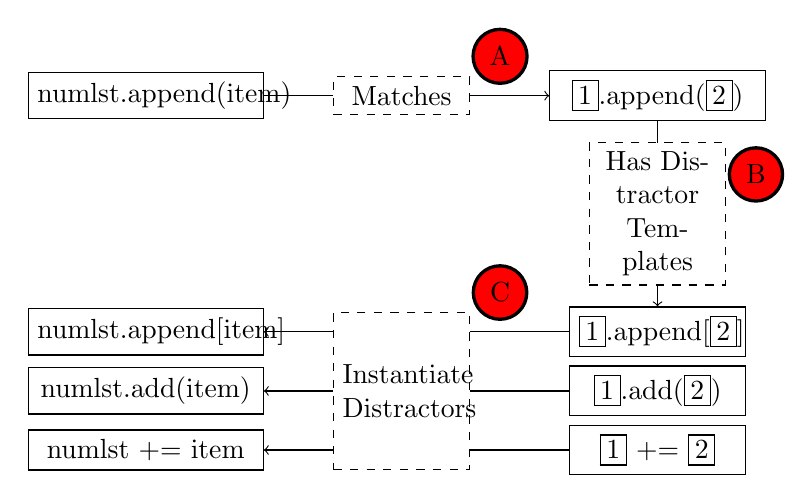
\begin{tikzpicture}[node distance=2cm]

    \node (line) [draw, text width=2.75cm, align=center] {numlst.append(item)};
    \node (extract) [draw, xshift=4.5cm, right of=line, text width=2.5cm, align=center] {\boxed{1}.append(\boxed{2})};

    \node (d1struct) [draw, yshift=-1cm, below of=extract,    text width=2cm, align=center]   {\boxed{1}.append[\boxed{2}]};
    \node (d2struct) [draw, yshift=1.25cm, below of=d1struct, text width=2cm, align=center] {\boxed{1}.add(\boxed{2})};
    \node (d3struct) [draw, yshift=1.25cm, below of=d2struct, text width=2cm, align=center] {\boxed{1} += \boxed{2}};

    \node (d1) [draw, yshift=-1cm, below of=line, text width=2.75cm, align=center] {numlst.append[item]};
    \node (d2) [draw, yshift=1.25cm, below of=d1, text width=2.75cm, align=center]       {numlst.add(item)};
    \node (d3) [draw, yshift=1.25cm, below of=d2, text width=2.75cm, align=center]       {numlst += item};

    % Arrows
    \draw[->] (line.east) -- (extract.west);
    \draw[->] (extract) -- (d1struct);
    \draw[->] (d1struct.west) -- (d1.east);
    \draw[->] (d2struct.west) -- (d2.east);
    \draw[->] (d3struct.west) -- (d3.east);

    % Transition labels
    \node (matches) [fill=white, xshift=1.25cm, right of=line, draw, text width=1.5cm, align=center, dashed] {Matches};
    \node (hasdist) [fill=white, yshift=0.5cm, below of=extract, draw, text width=1.5cm, align=center, dashed] {Has Distractor Templates};
    \node (instantiate) [text centered, fill=white, xshift=-1.25cm, left of=d2struct, draw, text width=1.5cm, minimum height=2cm, dashed] {Instantiate\\ Distractors};

    % Labels
    \node (1) [draw, circle, right of=matches,     fill=red, very thick, xshift=-0.75cm, yshift=0.50cm] {A};
    \node (2) [draw, circle, right of=hasdist,     fill=red, very thick, xshift=-0.75cm, yshift=0.50cm] {B};
    \node (3) [draw, circle, right of=instantiate, fill=red, very thick, xshift=-0.75cm, yshift=1.25cm] {C};


\end{tikzpicture}


    }
    \caption{Transforming \texttt{numlst.append(item)} into a set of distractors.}
    \label{fig:appendastmatchesed}
\end{figure}

To enable the rapid authoring of questions that include distrators, we also 
developed a process of autogenerating distractors for a given, correct piece of code.
This is done by leveraging the errors we discovered through the previously
mentioned analysis process.  The process begins by one again constructing
partial ASTs for the correct form of each of the statements for which sets of
distractor templates were constructed.  For example, if we want to support
creating distractors for the append statement we would construct a partial AST
for \texttt{\boxed{1}.append(\boxed{2})}.  As shown in
Figure~\ref{fig:appendastmatchesed}, if a line of code is then entered that
matches this partial AST (e.g., \texttt{numlst.append(item)}) that match can
(A) be identified and (B) the set of distractor templates associated with the
matched statement can be retrieved. The final step (C) involves extracting and
unparsing the subtrees from the original line of code's AST that are occupied
by wildcards in the partial AST. These subtrees represent the values that will
be placed into their respective positions in the distractor templates in order
to generate the final set of distractors.

With this set of distractors collected and a process for generating them put in
place, we then performed a pilot study aimed at evaluating the impacts of including
distractors in Parsons problems on exams. In doing so, we created three pairs of items
were each pair had the same prompt and base solution but one version contained jumbled
distractors and the other did not. These questions were then randomly assigned to
students on a final exam in a large, introductory Python course.  We then
evaluated these items using the following metrics: 
\begin{enumerate}
  \item \textbf{Item-Discrimination:}
  \item \textbf{Item-Difficulty:}
  \item \textbf{Duration:}
\end{enumerate}

\paragraph{Results and Takeaways:}


\subsection{Evaluating Distractors}\label{sec:eval}

\paragraph{Abstract:} Since the creation of the tool for 

\paragraph{Methodology:}

\paragraph{Results and Takeaways:}

\section{Limitations of Prior Work}

The primary limitations of the prior work are threefold. First, the distractors 
being used are limited to those that can be generated from the errors students
make on statement questions used in the course. These are primarily limited to 
operations used to manipulate Python's builtin data structures. The results of 
the prior studies may differ if the distractors used focused on looping and 
conditional structures. For example, recent work by \citet{} found that 
blocks in faded (fill in the blank) Parsons problems that required students
to complete conditionals proved to be the most difficult.


Secondly, my prior work on using distractors in summative assessments 
failed to account for how the number of distractors groups present in a problem
impacts the results. The majority of problems in the prior studies only
contained either one or two groups of distractors. It may be the case that
a larger number of groups with a more diverse set of distractors leads to 
a more measurable increase in item quality. Conversely, it might also be the
case that by including more distractors the item experiences more ``slip'' 
and thus decreases the item quality. In either case, further investigations
are needed to identify the impacts of increasing the number of distractor 
groups present in a Parsons problem when used in summative assessments.


Finally, my prior work only evaluated the distractors in the context of
summative assessments. Though prior work has certainly indicated that
distractors are used in Parsons problems when they are used as an exam item,
the original intention of Parsons problems was as a exercise
tool~\cite{parsons2006parson} and is often discussed as being used as a method
for transitioning students into writing code. As such, though my prior work
makes tentative steps towards informing the use of distractors in summative
assessments, it leaves open the door for further investigation into the impact
of distractors on learning outcomes when used in formative contexts.

\section{Ongoing and Future Work}

In addressing the limitations of the completed work, we propose three research
directions:
\begin{enumerate}
  \item[RD1)] Developing a more complete taxonomy of distractors from errors
    students make on statement questions \textbf{and} write code question in support of
    RD1 and RD2 (Section~\ref{sec:taxonomy}).
  \item[RD2)] A larger study, over multiple semesters, on the impact of distractors on the psychometric
    properties of Parsons problems as exam items (Section~\ref{sec:itemquality}).
  \item[RD3)] Investigating the impact of distractors on learning outcomes in a
    variety of CS contexts (Section~\ref{sec:impact}).
\end{enumerate}
Each of these proposed directions. 

\subsubsection{RD1) Building a Taxonomy of Distractors for Python}\label{sec:taxonomy}

This proposed work stems from the prior work initially described in
Section~\ref{sec:creation}. We will extend the analysis performed on statement questions to
include errors and categories of errors students make on code writing activities
in order to create a more complete set of distractors from which a more
generalized taxonomy will be built. 

\paragraph{Methodology:} In the introductory programming course from which
the data for the first paper detailed in \ref{sec:creation} was attained
we have a variety large quantity of historical data. Though in that analysis
we focused on collecting data from ``statement questions'' we also have a wide
variety 

\paragraph{Expected Outcomes:} The primary deliverable of this study will be
the taxonomy and bank of common errors itself. The utility of this is twofold.
First, it can be used as a guidebook for question authoring. Second, it can be
used in future anlaysis of distractors to guide how they can be used in
summative and formative contexts alike.

\paragraph{Timeline:} 


\subsubsection{RD2) Investigating the Impact of Distractors on Learning Outcomes in CS1}\label{sec:impact}}

The second research direction (Section~\ref{impact}) will investigate the impact
of distractors on learning outcomes in a CS1 context. This will consist of a
series of A-B studies comparing the performance of students on posts tests after
learning from Parsons problems with and without distractors. These studies will
additionally include a series of interviews with students completing the
problems to determine if the distractors provide any additional benefit to the
students beyond potential learning gains. 

\paragraph{Methodology:} In answering the research questions above we use a mixed 
methods approach.
To evaluate the research questions listed above we ran 
and A-B comparing the learning gains of students practicing with and without distractors.
In both conditions students began by completing a short reading on a topic they had 
not encountered in the course, in this case Pythons sorting functions. They then
completed a survey on their familiarity with the functions they read about prior
to completing the reading. 

\paragraph{Expected Outcomes:} 

\paragraph{Timeline:} The data collection for the quantitative portion of this
study has already been completed and had undergone preliminary analysis. Several 
interviews have been conducted with students with more currently underway. We are 
targeting ICER 2024 for the publication of this work.
 
\subsubsection{RD3) An Extended Analysis of the Impact of Distractors on Exam Items }\label{sec:itemquality}

The third and final research direction (Section~\ref{itemquality}) will
invovle a long term continuation of the work described in Section~\ref{eval}.
A core limitation of this prior work is there are a number of ways in which 
distractors can be inlcuded in an exam item. For example, multiple groups 
of visually grouped distractors can be included in a single item, the number 
of distractors per group can be varied, and there are a variety of distractor 
types which can be included. This research direction will involve the development
of a wide variety of Parsons problems with these parameters varied and anlaysing
the impact of these parameters on the quality of the exam items.

\paragraph{Methodology:} In the Fall 2023 semester we repeated the experiments
comparing Parsons problems with no distractors to those that included jumbled
and visually grouped distractors. In this iteration of the experiment we
constructed problems XXX sets of problems. Each set contained four problems
containing zero to three groups of distractors, respectively. Otherwise, each
had the same prompt and base solution and only differed in the number of
distractors which were included. These questions were randomly assigned to
students on exams and quizzes throughout the semester. We perform CTT and IRT
analysis to compare the difficulty and discrimination based on the number of
distractors present in the question. We additionally use the estimated viewing
times on PrairieLearn to determine how the amount of time students spent on the
questions differed based on the number of distractors the Parsons problem
contained. This experiment will be run over the next two semesters in an 
effort to collect a large and diverse set of problems.


\paragraph{Expected Outcomes:} One of the primary limitations of the prior work
is that it didn't pay sufficient attention to how the number of distractor 
groups in the problem may impact the difficulty, discrimination, and duration
statistics associated with the problem. The majority of questions from those 
analysis's 

\paragraph{Current Progress and Timeline:} 
An initial anlaysis of the Fall 2023 data has been analyzed and submitted to
ITiCSE 2024. The full analysis will include a replication of these initial
findings and a more indepth analysis of which distractors were the most
``distracting'' and how these item statistics differ for items included on
exams at different points in the semester.



\bibliographystyle{ACM-Reference-Format}
\balance
\bibliography{acmart}

\end{document}
\endinput
